\documentclass{article}
\usepackage{graphicx}
\usepackage{fancyhdr}
\usepackage{latexsym}
\usepackage{float}
\usepackage{caption}
\usepackage{amsmath}
\usepackage{hyperref}
\usepackage{geometry}
\usepackage{enumitem}
\usepackage{tikz}
\usetikzlibrary{positioning, matrix, arrows.meta}
\usepackage{adjustbox} % For scaling

\setlength{\parindent}{0pt}
\geometry{a4paper,scale=0.80}
\begin{document}
\textbf{9.6  Your university is holding a fund-raiser and will be hiring a band to entertain spectators.}\\[0.2em]
\hspace*{0.6cm}
\begin{minipage}{0.94\textwidth}
    \textbf{You have been selected to serve as the event project manager and have created a Work Breakdown Structure and duration estimates for the activities involved in site preparation for the event. Construct a network activity diagram based on the following information:}
\end{minipage}
\begin{table}[h!]
    \centering
    \begin{tabular}{|c|c|c|c|}
    \hline
    \textbf{Activity} & \textbf{Description}                 & \textbf{Predecessors} & \textbf{Duration (Days)} \\ \hline
    A                 & Site selection                       & None                  & 4                        \\ \hline
    B                 & Buy concessions                      & A                     & 4                        \\ \hline
    C                 & Rent facilities                      & A                     & 2                        \\ \hline
    D                 & Build Stands                         & A                     & 5                        \\ \hline
    E                 & Generator \& wiring installation     & C                     & 2                        \\ \hline
    F                 & Security                             & B                     & 4                        \\ \hline
    G                 & Lighting installation                & E                     & 2                        \\ \hline
    H                 & Sound system installation            & E, F                  & 2                        \\ \hline
    I                 & Stage construction                   & D                     & 3                        \\ \hline
    J                 & Tear down                            & G, H, I               & 4                        \\ \hline
    \end{tabular}
\end{table}\\
\hspace*{0.6cm}
\begin{minipage}{0.94\textwidth}
    \textbf{a. Conduct both a forward and backward pass using AON notation. What is the estimated total duration for the project?}\\[0.5em]
        \begin{adjustbox}{scale=0.68,center} % Adjust scale factor as needed
            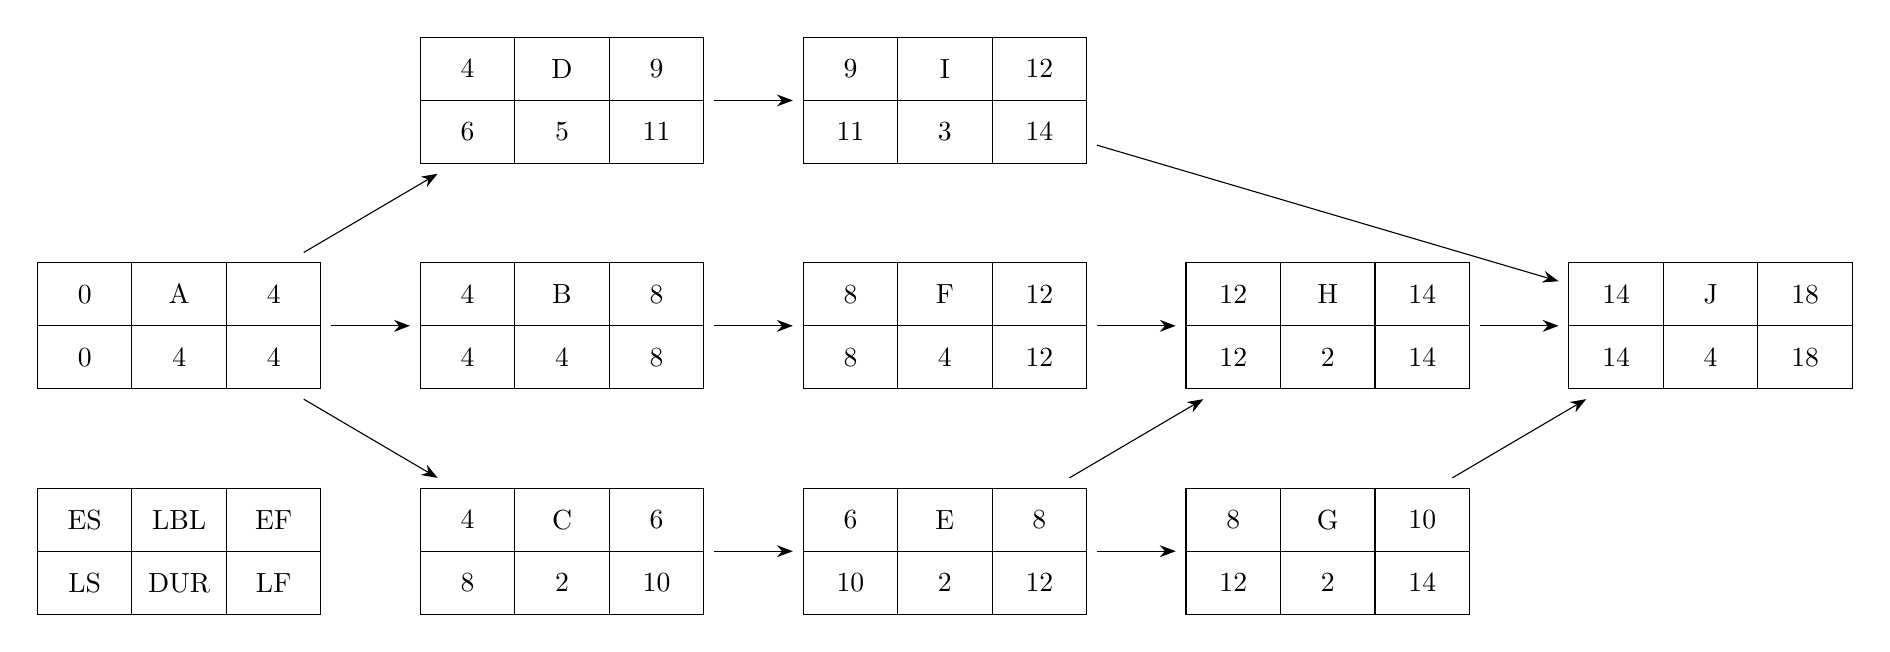
\begin{tikzpicture}[
                node distance=1cm and 1cm, 
                table/.style={
                  matrix of nodes,
                  nodes in empty cells,
                  nodes={draw, anchor=center, minimum width=1.2cm, minimum height=0.8cm},
                  column sep=-\pgflinewidth, row sep=-\pgflinewidth
                },
                arrow/.style={draw, -{Stealth[scale=1.2]}}
              ]
            
              \node (A) [table] { 0 & A & 4 \\ 0 & 4 & 4 \\ };
              \node (B) [table, right=of A] { 4 & B & 8 \\ 4 & 4 & 8 \\ };
              \node (C) [table, right=of A, below=of B] { 4 & C & 6 \\ 8 & 2 & 10 \\ };
              \node (D) [table, right=of B, above=of B] { 4 & D & 9 \\ 6 & 5 & 11 \\ };
              \node (E) [table, right=of C] { 6 & E & 8 \\ 10 & 2 & 12 \\ };
              \node (F) [table, right=of B] { 8 & F & 12 \\ 8 & 4 & 12 \\ };
              \node (I) [table, right=of D] { 9 & I & 12 \\ 11 & 3 & 14 \\ };
              \node (H) [table, right=of F] { 12 & H & 14 \\ 12 & 2 & 14 \\ };
              \node (G) [table, right=of E] { 8 & G & 10 \\ 12 & 2 & 14 \\ };
              \node (J) [table, right=of H] { 14 & J & 18 \\ 14 & 4 & 18 \\ };
              \node (EXP) [table, below=of A] { ES & LBL & EF \\ LS & DUR & LF \\ };
            
              % Draw arrows
              \draw[arrow] (A) -- (B);
              \draw[arrow] (A) -- (C);
              \draw[arrow] (A) -- (D);
              \draw[arrow] (D) -- (I);
              \draw[arrow] (B) -- (F);
              \draw[arrow] (C) -- (E);
              \draw[arrow] (F) -- (H);
              \draw[arrow] (E) -- (H);
              \draw[arrow] (E) -- (G);
              \draw[arrow] (I) -- (J);
              \draw[arrow] (H) -- (J);
              \draw[arrow] (G) -- (J);

            \end{tikzpicture}
            \end{adjustbox}
        from the above diagram, we can see that the estimated time to use is \textbf{\textit{18 Days}}. \\[1em]
    \textbf{b. Identify all paths through the network. Which is the critical path? Which activities have slack time?}\\[0.5em]
            The path without activities with slack time is the critical path, and for the diagram above, the critical path is:\\
            \begin{minipage}{\textwidth}
                \centering
                $A \rightarrow B \rightarrow F \rightarrow H \rightarrow J$
            \end{minipage}\\
        And we can have the below table showing the slack time for other activities:
\end{minipage}
    \begin{table}[h!]
        \centering
        \begin{tabular}{|c|c|}
        \hline
        \textbf{Activity} & \textbf{Days of Slack}\\ \hline
        C & 4 \\ \hline
        D & 2 \\ \hline
        E & 4 \\ \hline
        G & 4 \\ \hline
        I & 2 \\ \hline
        \end{tabular}
    \end{table}\\
  
\end{document}